\section{Implementation}
In this section, we show how we applied our idea of declarative style static
analysis for multilingual program to implement the proof-of-concept dataflow
analysis tool for JNI programs using CodeQL, which we named JN-QL. CodeQL is a
static analysis engine that transforms source code into database, and performs
analysis by evaluating "query", written in declarative language called QL
(Query Langague). In QL, defining rules are don via defining "predicates",
which has the following form:
\begin{lstlisting}[style=codeql,xleftmargin=2.5em]
predicate isOneTwoThree(int n) {
  n = 1
  or
  n = 2
  or
  n = 3
}
\end{lstlisting}

QL is also an object-oriented language, and it support class definition:
\begin{lstlisting}[style=codeql,xleftmargin=2.5em]
class OneTwoThree extends int {
  OneTwoThree() { // characteristic predicate
    this = 1
    or
    this = 2
    or
    this = 3
  }
}
\end{lstlisting}

Basically, defining class is not really different to defining predicate.  Class
is just set of elements that satisfy the predicate called "characteristic
prdicate". For more detailed information about QL, one can refer to the
paper[6] or the official document[7].

\begin{figure}[t]
  \centering
  \vspace{2mm}
  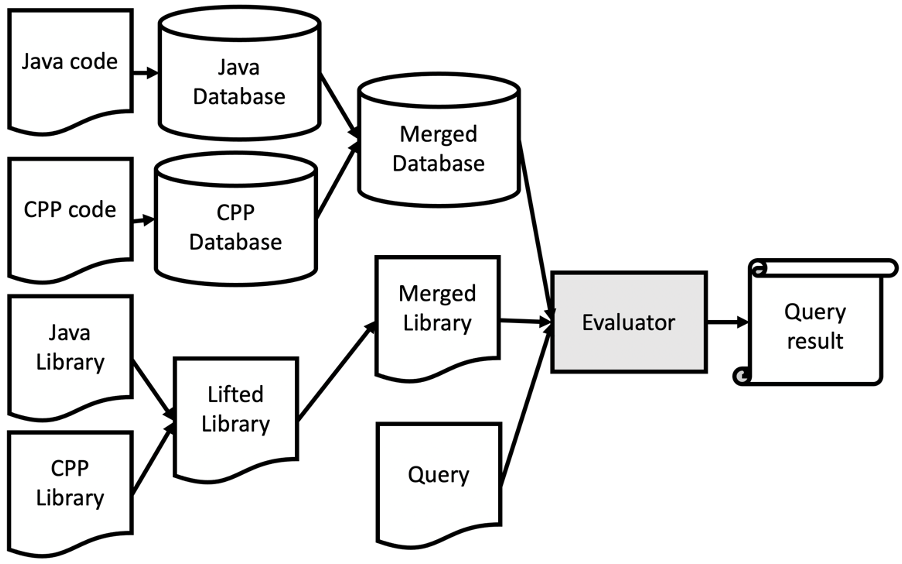
\includegraphics[width=0.5\textwidth]{img/Fig1}
  \vspace*{-1.5em}
  \caption{the overview of how declarative style analysis can be
  extended to multilingual analysis}
  \label{fig:Fig1}
\vspace*{-.5em}
\end{figure}

Figure~\ref{fig:Fig1} shows the overall structure of JN-QL. First, it generates database
for each language, C++ and Java, and merge it to one database. This corresponds
to a step of extracting syntactic data-facts from the source code. Then, we
merge two existing dataflow analysis framework, which are part of the library
that CodeQL provides as a form of library, into one merged library. Finally,
using the merged database and merged library, the user can write a query to
perform the client-analysis, and evaluate it to get analysis result.

\subsection{Create database}
The first step is to gernerate database for each of two languages.  For
compiled languages such as C++ and Java, CodeQL generates database by running
the compiler for each language. While the compiler is running, CodeQL monitors
the behavior of compiler and extracts information it needs, and create database
with that information.  Creation of database for one language is performed in
two steps: first, the extracted information from compiler is stored in the
human readable file format called trap files, and second, these trap files are
then finalized into database, written in binary format.

\inred{TODO: Explain this code briefly with caption?}
\begin{lstlisting}[style=java,numbers=none,xleftmargin=2.5em]
//Example of trap file
#10017=@"class;hello.HelloJNI"
...
#10044=@"type;int"
primitives(#10044,"int")
...
#10061=@"callable;{#10017}.java_callback({#10044}){#10044}"
...
#10067=@"params;{#10061};0"
params(#10067,#10044,0,#10061,#10067)
paramName(#10067,"java_callback_param")
\end{lstlisting}

In order to create a database for two languages, JN-QL performs first step for
each languages separately to get two sets of trap files.  Next step would be to
perfrom finalization step on merged set of trap files. However, a problem is that
both of trap files have table with duplicated name, so simply mering them would not work.
The solution is to add prefix to name of each table. For example, if both
database have tables named "@expr", the table from C++ would be renamed as
"@cpp\_expr", and the table from Java would be renamed as "@java\_expr". After
renaming each table, the second step can be applied to finalize the database on
which the query can be evaluated.

\subsection{Lift library}
CodeQL provides various libraries for each languages, which consists of some
pre-defined predicates and classes that can be useful for user to implement
analysis on their own taste. Dataflow analysis library is one of them, and both
C++ and Java supports this dataflow anslysis library. Two dataflow analysis
library have same framework: they share same classes such as "Node", and some
predicates such as "simpleLocalFlowStep".

\begin{lstlisting}[style=codeql,xleftmargin=2.5em]
// cpp/dataflow/internal/DataFlowUtil.qll
class Node extends TNode {
  ...
}
predicate simpleLocalFlowStep(Node nodeFrom, Node nodeTo) {
  // Expr -> Expr
  exprToExprStep_nocfg(
    nodeFrom.asExpr(),
    nodeTo.asExpr()
  )
  or
  // Assignment -> LValue post-update node
  ...
}
class Node extends TNode {
  ...
}
// java/dataflow/internal/DataFlowUtil.qll
predicate simpleLocalFlowStep(Node node1, Node node2) {
  // Variable flow steps through
  // adjacent def-use and use-use pairs.
  exists(SsaExplicitUpdate upd |
    upd.getDefiningExpr().(VariableAssign).getSource()
    = node1.asExpr() or
    upd.getDefiningExpr().(AssignOp) = node1.asExpr()
  |
    node2.asExpr() = upd.getAFirstUse()
  )
  or
  // Flow through this
  ...
}
\end{lstlisting}
However, these two implementations are not compatible, that is, although they have the same name,
we can not use "Node" class of C++ as an argument for "simpleLocalFlowStep" predicate of Java or vice versa.
Therefore, we lift each of the library into the same level so that classes and predicates become compatible.
First, we encapsulated each of original dataflow into CodeQL's module, named CPP and JAVA so that
original classes and predicated can be distinguished with lifted ones.
A class can be lifted by first defining sum type, which denotes that the lifted class would be either from C++ or
Java, and then make the lifted class be of that type. We also implemented two member predicates that can cast
the lifted class into each of corresponding class.
\begin{lstlisting}[style=codeql,xleftmargin=2.5em]
private newtype TNode =
  TJavaNode(JAVA::Node n)
  or
  TCppNode(CPP::Node n)
class Node extends TNode {
  JAVA::Node asJava() {
    this = TJavaNode(result)
  }
  CPP::Node asCpp() {
    this = TCppNode(result)
  }
  ...
}
\end{lstlisting}

A predicate can be lifted by combining two original predicates with "or"
connectives.  For each original predicate, each of the arguments and return
values are casted down to correspnding language's class. After lifting, the
lifted predicate shows equlivalent behavior as the original ones if all the
arguments are from the same language.
\begin{lstlisting}[style=codeql,xleftmargin=2.5em]
predicate simpleLocalFlowStep(Node node1, Node node2) {
  JAVA::simpleLocalFlowStep(
    node1.asJava(), node2.asJava()
  )
  or
  CPP::simpleLocalFlowStep(
    node1.asCpp(), node2.asCpp()
  )
}
\end{lstlisting}
\subsection{Merge library}

After the library is lifted, the last step is to extend some predicates to
reflect the semantics of interoperation between languages. The interaction from
Java to C, or C to Java are identified, and some predicates are extended to
model their behaviors. As an concrete exmpale, Let's take a look how the predicate
named viableCallable can be extended.
\begin{lstlisting}[style=codeql,xleftmargin=2.5em]
DataFlowCallable viableCallable(DataFlowCall c) {
result.asJava()
  = JAVA::viableCallable(c.asJava()) or
result.asCpp()
  = CPP::viableCallable(c.asCpp()) or
result.asCpp()
  = viableCallableJ2C(c.asJava()) or
result.asJava()
  = viableCallableC2J(c.asCpp())
}
\end{lstlisting}
The first two lines are result of lifting, and they take advantage of the
original predicates from dataflow library.  They handle the call edges from
Java to Java, and from C to C.

Next two lines are the result of merging library, and they are responsible for
inter-language call edges.  The predicate "viableCallableJ2C" finds call edges
from Java to C++, and the predicate "viableCallableC2J" finds call edges from
C++ to Java. These two call edges have different characteristic, and they
are implemented in different way.

\textbf{Java to C} The interaction from Java to C is done by Java code
calling native function in C, possibly with some arguments. The function
call target is determined in static manner. The target function should
follow the JNI naming convention, which is adding "Java\_" as prefix, 
folowed by fully qualified name of class and additional "\_", to the
method name. For example, the target function name for the method call
cfunction would be Java\_fully\_\_qualified\_\_class\_\_name\_cfunction.
Based on this convenvtion, we can define the predicate viableCallableJ2C
so that f = viablaCallableJ2C(m) holds when f.toString() = "Java\_" + 
m.className() + "\_" + "m.toString() holds. \inred{Include concrete code?}

\textbf{C to Java} The interaction from C to Java is more complex, and
requires more detailed implementation. The biggest difference is that
the method call from C to Java requires the runtime value of variables.
First, C calls the interface function "GetMethodID(name, sig)" to get "method
ID" of the method whooe name mathces the first argument, and the type signature
matches the second argument passed to this function. This method id is stored
at a variable, say "mid", and actual method call is done by calling another
interface function, "Call<type>Method(obj, mid, args...)". Calling this interface
function corresponds to call the method that mid indicates, with the "this object" as
obj, and the arguments as args.

In order to correctly handle this method call, we have to answer these
questions: "what string values does 'name' or 'sig' have when GetMetodID is
called", and "what method ID value does 'mid' have when Call<type>Method is
called". Note that what we need to answer to this question is the dataflow
analysis. Although inter-language dataflow is needed to soundly answer to the
questions, in practice intra-languae dataflow analysis is enough in most
situatitions. Therefore, we implemented two "inner-flow" analysis module for C,
which find all the dataflow from string literal to the argument of interface
function, and the dataflow from interface function call result to the argument
of interface function. Based on these two modules, we can implement the
predicate viableCallableC2J by connecting the calledge from "Call<type>Method"
call to the method m, if there is a flow to mid from call to "GetMethodID", and
string values that flow into name argument and sig argument of the "GetMethodID"
corresponds with that of method m.
\inred{Include concrete code?}

Other than the predicate viableCallable, there are also other predicates that
are extended. Most of them are specialized "step" predicates, where the purpose
of extension is to consider other JNI interface functions, such as
findClass or GetFieldID. The extensions are done in similar as handling
call from C to Java mentioned above.
